%%%%%%%%%%%%%%%%%%%%%%%%%%%%%%%%%%%%%%%%%
% Beamer Presentation
% LaTeX Template
% Version 1.0 (10/11/12)
%
% This template has been downloaded from:
% http://www.LaTeXTemplates.com
%
% License:
% CC BY-NC-SA 3.0 (http://creativecommons.org/licenses/by-nc-sa/3.0/)
%
%%%%%%%%%%%%%%%%%%%%%%%%%%%%%%%%%%%%%%%%%

%----------------------------------------------------------------------------------------
%	PACKAGES AND THEMES
%----------------------------------------------------------------------------------------

\documentclass{beamer}

%----------------------------------------------------------------------------------------
%	IMPORTACIONES
%----------------------------------------------------------------------------------------

\usepackage{amssymb}% http://ctan.org/pkg/amssymb
\usepackage{pifont}% http://ctan.org/pkg/pifont
\newcommand{\cmark}{\ding{51}}%
\newcommand{\xmark}{\ding{55}}%

%paquete usado para silabación en español
\usepackage[spanish]{babel}
%codificación del documento
\usepackage[utf8]{inputenc}

\mode<presentation> {

% The Beamer class comes with a number of default slide themes
% which change the colors and layouts of slides. Below this is a list
% of all the themes, uncomment each in turn to see what they look like.

%\usetheme{default}
%\usetheme{AnnArbor}
%\usetheme{Antibes}
%\usetheme{Bergen}
%\usetheme{Berkeley}
\usetheme{Berlin}
%\usetheme{Boadilla}
%\usetheme{CambridgeUS}
%\usetheme{Copenhagen}
%\usetheme{Darmstadt}
%\usetheme{Dresden}
%\usetheme{Frankfurt}
%\usetheme{Goettingen}
%\usetheme{Hannover}
%\usetheme{Ilmenau}
%\usetheme{JuanLesPins}
%\usetheme{Luebeck}
%\usetheme{Madrid}
%\usetheme{Malmoe}
%\usetheme{Marburg}
%\usetheme{Montpellier}
%\usetheme{PaloAlto}
%\usetheme{Pittsburgh}
%\usetheme{Rochester}
%\usetheme{Singapore}
%\usetheme{Szeged}
%\usetheme{Warsaw}

% As well as themes, the Beamer class has a number of color themes
% for any slide theme. Uncomment each of these in turn to see how it
% changes the colors of your current slide theme.

%\usecolortheme{albatross}
%\usecolortheme{beaver}
%\usecolortheme{beetle}
%\usecolortheme{crane}
%\usecolortheme{dolphin}
%\usecolortheme{dove}
%\usecolortheme{fly}
%\usecolortheme{lily}
%\usecolortheme{orchid}
%\usecolortheme{rose}
%\usecolortheme{seagull}
%\usecolortheme{seahorse}
%\usecolortheme{whale}
%\usecolortheme{wolverine}

%\setbeamertemplate{footline} % To remove the footer line in all slides uncomment this line
%\setbeamertemplate{footline}[page number] % To replace the footer line in all slides with a simple slide count uncomment this line

%\setbeamertemplate{navigation symbols}{} % To remove the navigation symbols from the bottom of all slides uncomment this line
}

\usepackage{graphicx} % Allows including images
\usepackage{booktabs} % Allows the use of \toprule, \midrule and \bottomrule in tables

%----------------------------------------------------------------------------------------
%	TITLE PAGE
%----------------------------------------------------------------------------------------

\title[SEPA 2.0]{MÓDULOS INTEGRADOR Y MANTENEDOR DE DATOS EN SISTEMA SEPA VERSION 2.0} % The short title appears at the bottom of every slide, the full title is only on the title page

\author{Miguel Ángel Aníbal Davor Fuenzalida Pino} % Your name
\institute[UTEM] % Your institution as it will appear on the bottom of every slide, may be shorthand to save space
{
UNIVERSIDAD TECNOLÓGICA METROPOLITANA \\ % Your institution for the title page
\medskip
\textit{anibaldavor@gmail.com} % Your email address
}
\date{\today} % Date, can be changed to a custom date

\begin{document}

\begin{frame}
\titlepage % Print the title page as the first slide
\end{frame}

\begin{frame}
\frametitle{Contenidos} % Table of contents slide, comment this block out to remove it
\tableofcontents % Throughout your presentation, if you choose to use \section{} and \subsection{} commands, these will automatically be printed on this slide as an overview of your presentation
\end{frame}

%----------------------------------------------------------------------------------------
%	PRESENTATION SLIDES
%----------------------------------------------------------------------------------------

\section{Análisis}

\subsection{Resumen}

\begin{frame}
\frametitle{SEPA Anterior}
\begin{itemize}
\item Datos probenientes de DirDoc, proceso de traspaso inseguro.
\item Carece de formas alternativas de acceso.
\item Falta de roles para los usuarios.
\item No es posible reparar datos incompletos.
\end{itemize}
\end{frame}

%------------------------------------------------

\begin{frame}
\frametitle{SEPA Nuevo}
\begin{itemize}
\item Mantenedor: Versión actualizada de SEPA.
\item Integrador: Rescate de información automático.
\end{itemize}
\end{frame}

%------------------------------------------------

\begin{frame}
\frametitle{Beneficios}
\begin{itemize}
\item Información que otorga una mejor perspectiva de la realidad universitaria.
\item Mirar el desempeño académico de un estudiante.
\item Integrar componentes o funcionalidades a SEPA 2.0.
\item Extracción de data en forma segura y automática.
\end{itemize}
\end{frame}

%------------------------------------------------

\begin{frame}
\frametitle{Situación final}
\begin{itemize}
\item Ingreso por perfiles.
\item Visualización de todas las tablas que componen la base de datos.
\item Mantenedor de perfiles.
\item Web Service integrador.
\item Expansibilidad.
\end{itemize}
\end{frame}

%------------------------------------------------

\subsection{Proceso}

\begin{frame}
\frametitle{Objetivos}
\begin{block}{General}
Actualizar SEPA a una versión 2.0, creando un sistema actualizado e independiente de información estadística para la Universidad Tecnológica Metropolitana ayudando a sus procesos docentes y productivos, disponiendo de información veraz a la realidad universitaria.
\end{block}


\begin{itemize}
\item Sistema simple de mejorar.
\item Desarrollado bajo herramientas robustas.
\item Creación de un SEPA 2.0 diferente de su predecesor.
\end{itemize}
\end{frame}

%------------------------------------------------

\begin{frame}
\frametitle{Diagrama del proyecto}
\begin{figure}[!hbp]
\begin{center}
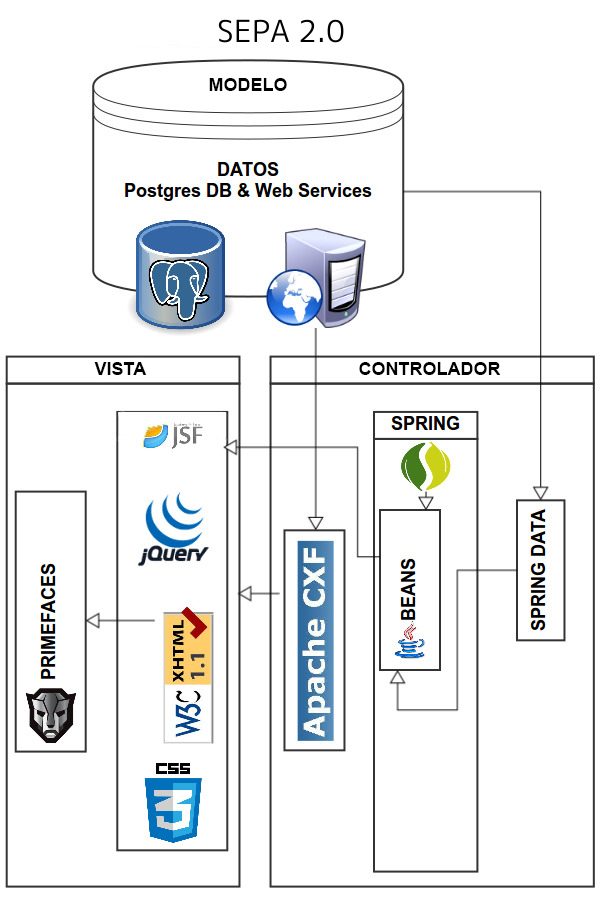
\includegraphics[scale=0.2,angle=0]{images/diagrama2.jpg}
\caption{Diagrama general del sistema}
\label{Diagrama general del sistema}
\end{center}
\end{figure}
\end{frame}

%------------------------------------------------

\begin{frame}
\frametitle{Ciclo de Vida}
\begin{figure}[!hbp]
\begin{center}
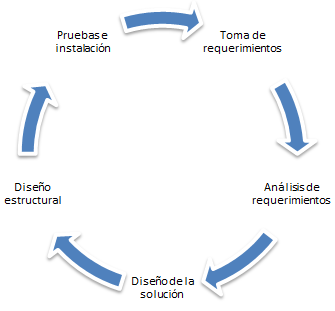
\includegraphics[scale=0.6,angle=0]{images/cicloMini.PNG}
\caption{Ciclo de vida}
\label{Organigrama de rectoria}
\end{center}
\end{figure}
\end{frame}

%------------------------------------------------

\begin{frame}
\frametitle{Estado del Arte}
\begin{block}{QS Top Universities}
Evaluación mediante ránkings enfocados a entregar información a organismos y personas relacionadas con post-grados, MBA, estudios de ingeniería y negocios.
\end{block}
\begin{block}{Ránking de Calidad de las Universidades Chilenas}
Ránking para instituciones educacionales en Chile, que utiliza ciertos criterios, como son la cantidad de investigaciones o la masa de estudiantes que entran en cada Universidad.
\end{block}
\end{frame}

%------------------------------------------------

\begin{frame}
\frametitle{Análisis de las Herramientas}
\begin{table}
\begin{tabular}{l l l l l}
\toprule
				& \textbf{php} & \textbf{.net} & \textbf{Rails} & \textbf{Java}\\
\midrule
Sencillez 		& \textcolor{green}{\cmark} & \textcolor{red}{\xmark}   & \textcolor{red}{\xmark}   &\textcolor{green}{\cmark}\\
Robustez 		& \textcolor{red}{\xmark}   & \textcolor{green}{\cmark} & \textcolor{green}{\cmark} &\textcolor{green}{\cmark}\\
Seguridad 		& \textcolor{red}{\xmark}   & \textcolor{red}{\xmark}   & \textcolor{green}{\cmark} &\textcolor{green}{\cmark}\\
Portabilidad 	& \textcolor{green}{\cmark} & \textcolor{red}{\xmark}   & \textcolor{red}{\xmark}   &\textcolor{green}{\cmark}\\
Neutralidad 	& \textcolor{green}{\cmark} & \textcolor{red}{\xmark}   & \textcolor{green}{\cmark} &\textcolor{green}{\cmark}\\
Interfaz 		& \textcolor{red}{\xmark}   & \textcolor{green}{\cmark} & \textcolor{green}{\cmark} &\textcolor{green}{\cmark}\\
Expresividad 	& \textcolor{green}{\cmark} & \textcolor{red}{\xmark}   & \textcolor{green}{\cmark} &\textcolor{red}{\xmark}\\
Compilación 	& \textcolor{green}{\cmark} & \textcolor{red}{\xmark}   & \textcolor{green}{\cmark} &\textcolor{red}{\xmark}\\
Aprendizaje 	& \textcolor{green}{\cmark} & \textcolor{red}{\xmark}   & \textcolor{green}{\cmark} &\textcolor{green}{\cmark}\\
E. de control 	& \textcolor{green}{\cmark} & \textcolor{green}{\cmark} & \textcolor{green}{\cmark} &\textcolor{green}{\cmark}\\
Abstracción 	& \textcolor{green}{\cmark} & \textcolor{red}{\xmark}   & \textcolor{red}{\xmark}   &\textcolor{green}{\cmark}\\
\textbf{Total}  & 8 & 3 & 8 & 9\\
\bottomrule
\end{tabular}
\caption{Table caption}
\end{table}
\end{frame}

%------------------------------------------------

\section{Proyecto}

\subsection{Preámbulo}

%------------------------------------------------

\begin{frame}
\frametitle{Criterios de Calidad}
\begin{itemize}
\item \textbf{Mantenibilidad}: Modelo de programación simple para corregir.
\item \textbf{Flexibilidad}: Capacidad de crecimiento del código.
\item \textbf{Testeabilidad}: Test de funcionamiento.
\item \textbf{Portabilidad}: Portabilidad sobre muchos S.O. en distintas arquitecturas
\item \textbf{Integridad}: Integridad de la data que es ingresada.
\item \textbf{Rapidez}: Ejecución de servicios de forma veloz y clara.
\end{itemize}
\end{frame}

%------------------------------------------------

\begin{frame}
\frametitle{Patrones de Diseño}
\begin{itemize}
\item \textbf{MVC}: Modelo Vista Controlador
\item \textbf{SOA}: Arquitectura orientada a servicios
\item \textbf{POA}: Programación Orientada al Aspecto
\item \textbf{DAO}: Objeto de Acceso a datos
\end{itemize}
\end{frame}

\subsection{Desarrollo}

%------------------------------------------------

\begin{frame}
\frametitle{Integrador}
\begin{itemize}
\item \textbf{Poblador}: Herramienta desarrollada con el fin de buscar los datos desde DirDoc de manera segura y controlada.
\item \textbf{Periodicidad}: Característica del poblador que establece fechas, horas y minutos en donde varios servicios consultan datos.
\item \textbf{Web Service}: Framework que permite la comunicación entre 2 sistemas mediante un lenguaje de marcado expuesto por el que envia y el receptor.
\end{itemize}
\end{frame}

%------------------------------------------------

\begin{frame}
\frametitle{Operaciones}
\begin{itemize}
\item \textbf{Tarea Diaria}: Actualizar Cohortes y Estudiantes.
\item \textbf{Tarea Semanal}: Actualizar Asignaturas Cursadas.
\item \textbf{Tarea Mensual}: Actualizar Cursos, Docentes y Cargos.
\item \textbf{Tarea Trimestral}: Actualizar Asignaturas, Cupos Carreras y Titulados.
\item \textbf{Tarea Semestral}: Actualizar Establecimientos.
\item \textbf{Tarea Anual}: Actualizar Carreras, Planes de Estudio y Quintalización
\end{itemize}
\end{frame}

%------------------------------------------------

\begin{frame}
\frametitle{Tabla Comparativa (Integrador)}
\begin{table}
\begin{tabular}{l l l l}
\toprule
\textbf{SEPA} & \textbf{Hoy} & \textbf{2.0} & Característica\\
\midrule
Instalación 	& \textcolor{green}{\cmark} & \textcolor{green}{\cmark} & Servidor de aplicaciones  \\
Uso		 		& \textcolor{green}{\cmark} & \textcolor{green}{\cmark} & Uso automático \\
Monitoreo 		& \textcolor{red}{\xmark}   & \textcolor{green}{\cmark} & Genera alertas debido a fallos \\
Portabilidad 	& \textcolor{red}{\xmark}   & \textcolor{green}{\cmark} & Se puede reinstalar \\
Estabilidad 	& \textcolor{red}{\xmark}   & \textcolor{green}{\cmark} & Presenta pocos o nulos fallos \\
\bottomrule
\end{tabular}
\end{table}
\end{frame}

%------------------------------------------------

\begin{frame}
\frametitle{Mantenedor}
\begin{itemize}
\item Sitio Web
\item Perfiles
\item Ingreso
\end{itemize}
\end{frame}

%------------------------------------------------

\begin{frame}
\frametitle{Mantenedores}
\begin{itemize}
\item Inicio
\item Acceso
\item Geografía
\item Utem
\item Curso
\item Estudiante
\item Contacto
\item Sesión
\end{itemize}
\end{frame}

%------------------------------------------------

\begin{frame}
\frametitle{Tabla Comparativa (Mantenedor)}
\begin{table}
\begin{tabular}{l l l l}
\toprule
\textbf{SEPA} & \textbf{Hoy} & \textbf{2.0} & Característica\\
\midrule
Instalación 	& \textcolor{green}{\cmark} & \textcolor{green}{\cmark} & Servidor de aplicaciones  \\
Uso		 		& \textcolor{green}{\cmark} & \textcolor{green}{\cmark} & Uso automático \\
Monitoreo 		& \textcolor{red}{\xmark}   & \textcolor{green}{\cmark} & Genera alertas debido a fallos \\
Portabilidad 	& \textcolor{red}{\xmark}   & \textcolor{green}{\cmark} & Se puede reinstalar \\
Estabilidad 	& \textcolor{red}{\xmark}   & \textcolor{green}{\cmark} & Presenta pocos o nulos fallos \\
\bottomrule
\end{tabular}
\end{table}
\end{frame}

%------------------------------------------------

\section{Resultados} 

\subsection{Evaluación}

%------------------------------------------------

\begin{frame}
\frametitle{Estimación de Costos}
\begin{block}{COCOMO}
ASDF
\end{block}
\begin{block}{Punto Función}
asdf
\end{block}
\end{frame}

%------------------------------------------------

\begin{frame}
\frametitle{Conteo de puntos}
\begin{itemize}
\item tabla puntos
\end{itemize}
\end{frame}

%------------------------------------------------

\begin{frame}
\frametitle{Características Generales del Sistema}
\begin{itemize}
\item tabla y Calculo de puntos de Funcion ajustados
\end{itemize}
\end{frame}

%------------------------------------------------

\begin{frame}
\frametitle{Valor Final}
\begin{itemize}
\item calculo final
\end{itemize}
\end{frame}

%------------------------------------------------

\subsection{Conclusión}

%------------------------------------------------

\begin{frame}
\frametitle{Garantías de calidad}
\begin{itemize}
\item Postgre SQL
\item MyBatis - Spring Data
\item Web Service CXF
\item Primefaces JSF
\item MVC
\end{itemize}
\end{frame}

%------------------------------------------------

\begin{frame}
\frametitle{Conclusión Final}
Sed iaculis dapibus gravida. Morbi sed tortor erat, nec interdum arcu. Sed id lorem lectus. Quisque viverra augue id sem ornare non aliquam nibh tristique. Aenean in ligula nisl. Nulla sed tellus ipsum. Donec vestibulum ligula non lorem vulputate fermentum accumsan neque mollis.\\~\\

Sed diam enim, sagittis nec condimentum sit amet, ullamcorper sit amet libero. Aliquam vel dui orci, a porta odio. Nullam id suscipit ipsum. Aenean lobortis commodo sem, ut commodo leo gravida vitae. Pellentesque vehicula ante iaculis arcu pretium rutrum eget sit amet purus. Integer ornare nulla quis neque ultrices lobortis. Vestibulum ultrices tincidunt libero, quis commodo erat ullamcorper id.
\end{frame}

%------------------------------------------------

\begin{frame}
\frametitle{Trabajo Futuro}
Sed iaculis dapibus gravida. Morbi sed tortor erat, nec interdum arcu. Sed id lorem lectus. Quisque viverra augue id sem ornare non aliquam nibh tristique. Aenean in ligula nisl. Nulla sed tellus ipsum. Donec vestibulum ligula non lorem vulputate fermentum accumsan neque mollis.\\~\\

Sed diam enim, sagittis nec condimentum sit amet, ullamcorper sit amet libero. Aliquam vel dui orci, a porta odio. Nullam id suscipit ipsum. Aenean lobortis commodo sem, ut commodo leo gravida vitae. Pellentesque vehicula ante iaculis arcu pretium rutrum eget sit amet purus. Integer ornare nulla quis neque ultrices lobortis. Vestibulum ultrices tincidunt libero, quis commodo erat ullamcorper id.
\end{frame}

%------------------------------------------------
\section{First Section} % Sections can be created in order to organize your presentation into discrete blocks, all sections and subsections are automatically printed in the table of contents as an overview of the talk
%------------------------------------------------

\subsection{Subsection Example} % A subsection can be created just before a set of slides with a common theme to further break down your presentation into chunks

\begin{frame}
\frametitle{Paragraphs of Text}
Sed iaculis dapibus gravida. Morbi sed tortor erat, nec interdum arcu. Sed id lorem lectus. Quisque viverra augue id sem ornare non aliquam nibh tristique. Aenean in ligula nisl. Nulla sed tellus ipsum. Donec vestibulum ligula non lorem vulputate fermentum accumsan neque mollis.\\~\\

Sed diam enim, sagittis nec condimentum sit amet, ullamcorper sit amet libero. Aliquam vel dui orci, a porta odio. Nullam id suscipit ipsum. Aenean lobortis commodo sem, ut commodo leo gravida vitae. Pellentesque vehicula ante iaculis arcu pretium rutrum eget sit amet purus. Integer ornare nulla quis neque ultrices lobortis. Vestibulum ultrices tincidunt libero, quis commodo erat ullamcorper id.
\end{frame}

%------------------------------------------------

\begin{frame}
\frametitle{Bullet Points}
\begin{itemize}
\item Lorem ipsum dolor sit amet, consectetur adipiscing elit
\item Aliquam blandit faucibus nisi, sit amet dapibus enim tempus eu
\item Nulla commodo, erat quis gravida posuere, elit lacus lobortis est, quis porttitor odio mauris at libero
\item Nam cursus est eget velit posuere pellentesque
\item Vestibulum faucibus velit a augue condimentum quis convallis nulla gravida
\end{itemize}
\end{frame}

%------------------------------------------------

\begin{frame}
\frametitle{Blocks of Highlighted Text}
\begin{block}{Block 1}
Lorem ipsum dolor sit amet, consectetur adipiscing elit. Integer lectus nisl, ultricies in feugiat rutrum, porttitor sit amet augue. Aliquam ut tortor mauris. Sed volutpat ante purus, quis accumsan dolor.
\end{block}

\begin{block}{Block 2}
Pellentesque sed tellus purus. Class aptent taciti sociosqu ad litora torquent per conubia nostra, per inceptos himenaeos. Vestibulum quis magna at risus dictum tempor eu vitae velit.
\end{block}

\begin{block}{Block 3}
Suspendisse tincidunt sagittis gravida. Curabitur condimentum, enim sed venenatis rutrum, ipsum neque consectetur orci, sed blandit justo nisi ac lacus.
\end{block}
\end{frame}

%------------------------------------------------

\begin{frame}
\frametitle{Multiple Columns}
\begin{columns}[c] % The "c" option specifies centered vertical alignment while the "t" option is used for top vertical alignment

\column{.45\textwidth} % Left column and width
\textbf{Heading}
\begin{enumerate}
\item Statement
\item Explanation
\item Example
\end{enumerate}

\column{.5\textwidth} % Right column and width
Lorem ipsum dolor sit amet, consectetur adipiscing elit. Integer lectus nisl, ultricies in feugiat rutrum, porttitor sit amet augue. Aliquam ut tortor mauris. Sed volutpat ante purus, quis accumsan dolor.

\end{columns}
\end{frame}

%------------------------------------------------
\section{Second Section}
%------------------------------------------------

\begin{frame}
\frametitle{Table}
\begin{table}
\begin{tabular}{l l l}
\toprule
\textbf{Treatments} & \textbf{Response 1} & \textbf{Response 2}\\
\midrule
Treatment 1 & 0.0003262 & 0.562 \\
Treatment 2 & 0.0015681 & 0.910 \\
Treatment 3 & 0.0009271 & 0.296 \\
\bottomrule
\end{tabular}
\caption{Table caption}
\end{table}
\end{frame}

%------------------------------------------------

\begin{frame}
\frametitle{Theorem}
\begin{theorem}[Mass--energy equivalence]
$E = mc^2$
\end{theorem}
\end{frame}

%------------------------------------------------

\begin{frame}[fragile] % Need to use the fragile option when verbatim is used in the slide
\frametitle{Verbatim}
\begin{example}[Theorem Slide Code]
\begin{verbatim}
\begin{frame}
\frametitle{Theorem}
\begin{theorem}[Mass--energy equivalence]
$E = mc^2$
\end{theorem}
\end{frame}\end{verbatim}
\end{example}
\end{frame}

%------------------------------------------------

\begin{frame}
\frametitle{Figure}
Uncomment the code on this slide to include your own image from the same directory as the template .TeX file.
%\begin{figure}
%\includegraphics[width=0.8\linewidth]{test}
%\end{figure}
\end{frame}

%------------------------------------------------

\begin{frame}[fragile] % Need to use the fragile option when verbatim is used in the slide
\frametitle{Citation}
An example of the \verb|\cite| command to cite within the presentation:\\~

This statement requires citation \cite{p1}.
\end{frame}

%------------------------------------------------

\begin{frame}
\frametitle{References}
\footnotesize{
\begin{thebibliography}{99} % Beamer does not support BibTeX so references must be inserted manually as below
\bibitem[Smith, 2012]{p1} John Smith (2012)
\newblock Title of the publication
\newblock \emph{Journal Name} 12(3), 45 -- 678.
\end{thebibliography}
}
\end{frame}

%------------------------------------------------

\begin{frame}
\Huge{\centerline{The End}}
\end{frame}

%----------------------------------------------------------------------------------------

\end{document} 